\documentclass{article}
\usepackage[utf8]{inputenc}

\title{Mobiele Data Communicatie}
\author{Jeffrey Gorissen}
\date{November 2018}

\usepackage[sort, numbers]{natbib}
\usepackage{graphicx}
\usepackage{float}
\usepackage[dutch]{babel}

\begin{document}

\begin{titlepage}
  
  \begin{flushright}
	  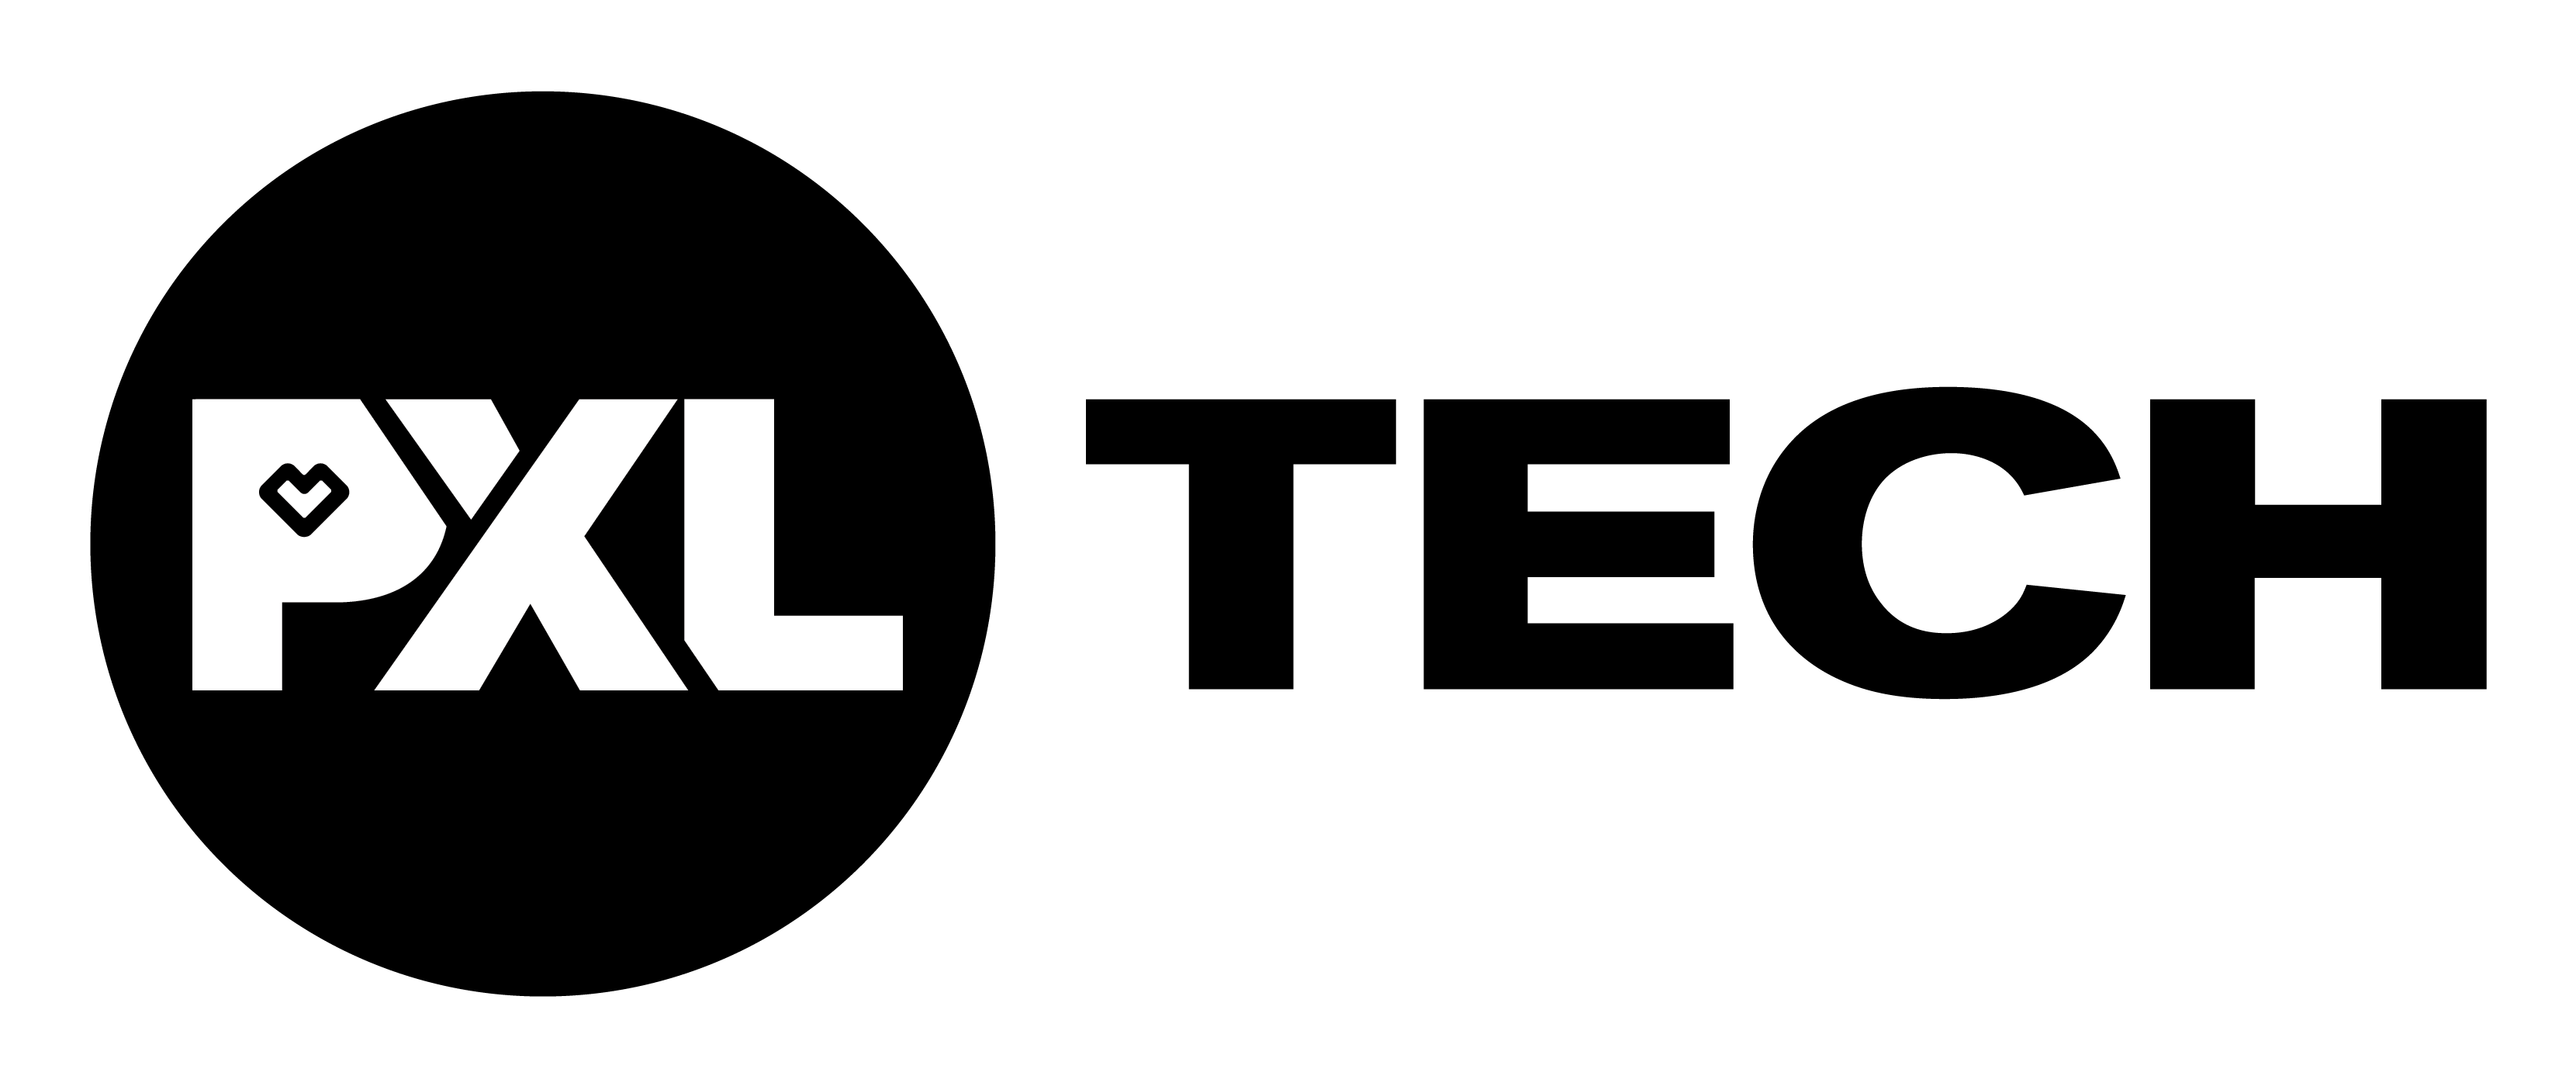
\includegraphics[width=6cm]{img/PXL-Tech.png}\\ 
    \Large 	Digitale Communicatie \\
    				Academiejaar 2018-2019\\
    				Ing. Dieter Vanrykel
  \end{flushright}
    \vspace*{\fill}
    		\begin{center}
      		\Huge \bf De evolutie van mobiele communicatieprotocollen \\en modulatie technieken:\\ 1G, 2G, 3G, 4G en 5G\\[3cm]
    		\end{center}
    \vspace*{\fill}
  \begin{flushright}
    \Large
        Jeffrey Gorissen\\
        \vspace{5mm} 
		3$^e$ Bachelor Elektronica-ICT\\
		 
  \end{flushright}
  
\end{titlepage}

\tableofcontents

\newpage

\section{Abstract}
De evolutie van de mobiele communicatie is er een die doorheen verschillende tijdperken gaat. Van analoge technieken uit het verleden doorheen de digitale revolutie tot een volledig gedigitaliseerd systeem.\\

\noindent De lezer zal een stuk geschiedenis van bijna vijf decennia doorlopen. Zo is de cellulaire communicatietechnologie zeer ver geëvolueerd. Elke fase bracht nieuwe en opwindende mogelijkheden en diensten bij de eindgebruiker. Het is ondertussen meer dan een eeuw geleden dat Graham Bell de telefoon uitvond. Tegenwoordig is het bellen slechts één van de vele functies. Steeds meer en meer wordt de nadruk op data gelegd. Doorheen de verschillende generaties zien we dat er steeds meer belang aan gehecht wordt.\\

\noindent In de eerste generatie spreken we nog van analoge technologie. Mensen kunnen elkaar bellen, ze kunnen tegelijkertijd met elkaar spreken en elkaar horen. Full-Duplex is realiteit.\\

\noindent Generatie twee maakt de mobiele communicatie digitaal. Data komt in het zicht maar de SMS (Short Message Service) is een van de belangrijkste doorbraken van de tweede generatie. De SMS is nog steeds een veel gebruikte toepassing.\\

\noindent Data neemt het roer over vanaf generatie drie. Datasnelheden zijn hoog en websites laden duurt geen minuten meer dankzij modernere modulatietechnieken. De prijzen zakken en de batterijduur neemt toe door de verbeteringen in lithografie technologie.\\

\noindent Vandaag de dag gebruiken de meeste mensen technologieën van de vierde generatie. Snel internet en laag energieverbruik behoren tot de kernwoorden van 4G. De mobiele communicatie komt kort in de buurt van de vaste internetverbindingen. De snelheid en latency kunnen echter nog beter, iets waar de vaste verbindingen nog heer en meester zijn.\\

\noindent Lage latency en super hoge download en upload snelheden zijn de beloftes van generatie vijf. De combinatie van meerdere technieken moeten deze beloftes waar maken. Voor de eerste praktijktesten moet men nog even wachten, de eerste commerciële 5G netwerken worden in 2020 verwacht. 

\newpage

\section{1G: Analoge mobiele netwerk}

Generatie 1 is in 1979 gelanceerd in Japan als opvolger van de Mobile Radio Telephone ook bekend als 0G. Apparaten van generatie 0 (Figuur \ref{fig:Moto}) zoals de auto telefoons van Motorola en Bell kwamen in 1946 tot stand. Deze apparaten maakten gebruik van half-duplex communicatielijnen. Men kon dus enkel spreken of enkel ontvangen. De meeste onder ons zullen een walkietalkie hierbij herkennen als voorbeeld. \cite{0G} \\

\begin{figure}[H]
\centering
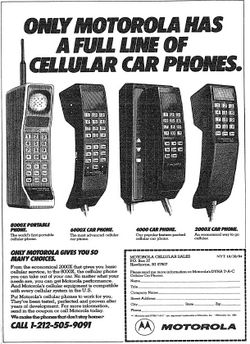
\includegraphics[width=0.85 \textwidth]{img/Moto.jpg}
\caption{Reclame auto telefoon Motorola.}
\label{fig:Moto}
\end{figure}

\subsection{De overgang van 0G naar 1G} \label{ssec: overgang}

\noindent We spreken bij 1G over een analoog netwerk. Indien men spreekt genereert men een geluidsgolf, dit is een analoog signaal. De 1G apparaten gebruikten natuurlijk geen geluid zoals de mens het ervaart. Ze gebruiken hiervoor analoge technologie om te communiceren op een bepaalde frequentieband. \\

\noindent Het communiceren over een bepaalde frequentieband gebeurd door de FDMA-techniek. Frequency division multiple access (FDMA) is een kanaal toegangs- of toewijzingsmethode die wordt gebruikt in protocollen met meerdere toegangen, zoals mobiele netwerken.\\

\noindent Met FDMA kunnen meerdere gebruikers (Mobiele telefoons) gegevens verzenden via een enkel communicatiekanaal, zoals een radio golf, door de bandbreedte van het kanaal te verdelen in afzonderlijke niet-overlappende frequentiesubkanalen en elk subkanaal toe te wijzen aan een afzonderlijke gebruiker (Zie Figuur \ref{fig:fdma}). Gebruikers kunnen gegevens verzenden via een subkanaal door het te moduleren op een draaggolf op de frequentie van het subkanaal. \cite{FDMA} \\

\begin{figure}[H]
\centering
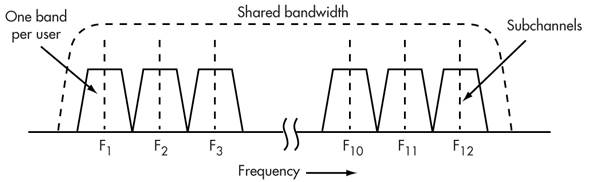
\includegraphics[width=0.9 \textwidth]{img/fdma.jpg}
\caption{Bandbreedte voor meerdere gebruikers met sub kanalen.}
\label{fig:fdma}
\end{figure}

\noindent In tegenstelling tot bij 0G is de communicatie bij 1G wel full-duplex. Mensen konden dus vanaf 1G elkaar horen en spreken tegelijkertijd. Verder was er geen operator, zie Figuur \ref{fig:operator}, meer nodig doordat de systemen rechtstreeks contact met elkaar konden opnemen. Bedrijven zoals Nokia en Motorola kwamen in 1970 met de eerste 1G apparaten op de markt. Rond het jaar 1981 werd er voor het eerst commercieel gebruikt gemaakt van deze apparaten. \cite{1G}

\begin{figure}[H]
\centering
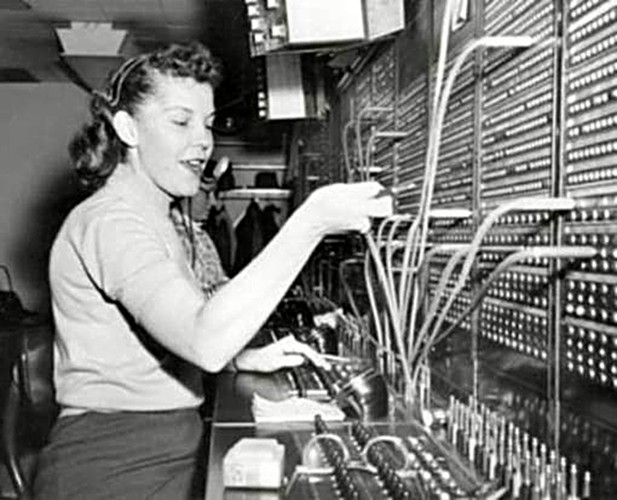
\includegraphics[width=0.7 \textwidth]{img/operator.jpg}
\caption{Telefoon operator.}
\label{fig:operator}
\end{figure}

\subsection{Modulatie techniek: Analoge FM}
De modulatie techniek die men in de eerste generatie gebruikte was analoge FM (Frequency Modulation). Frequentiemodulatie (FM) is het encoderen van informatie in een draaggolf door de frequentie van de golf te variëren. Bij analoge frequentiemodulatie is de frequentie-afwijking, het verschil tussen de frequentie van de draaggolf en zijn bron frequentie, evenredig aan het gemoduleerd signaal.\\

\noindent In de meest algemene vorm zal een FM-signaal er uit zien zoals in vergelijking \ref{eq:fm}. Hierbij is $V(t)$ de spanning van het signaal als functie van de tijd, $V_0$ de amplitude van het signaal, $f$ de oscillatie frequentie en $\phi$ de fase van het signaal die het startpunt van de cyclus representeert.

\begin{equation} \label{eq:fm}
    V(t) = V_o*sin (2\pi*f_t + \phi)
\end{equation}
\\
\noindent De modulatie van het signaal is als het ware een combinatie van de draaggolf met de gemoduleerde sinus golf. Dit resulteert in het FM-signaal. Op Figuur \ref{fig:modulatie} kan men een visuele weergave van het proces zien. 

\begin{figure}[H]
\centering
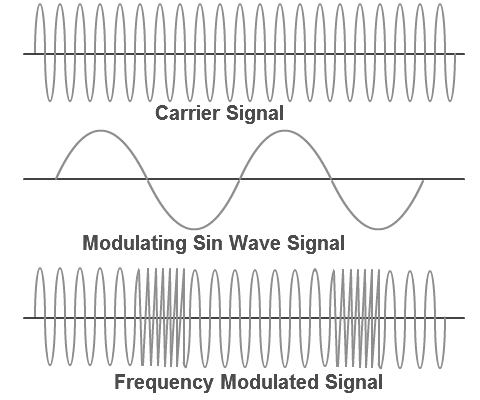
\includegraphics[width=0.85 \textwidth]{img/frequency-modulation.png}
\caption{Modulatie van een signaal}
\label{fig:modulatie}
\end{figure}


\subsection{Protocollen}

In deze subsectie bekijken we in het kort de drie bekendste protocollen die in de eerste generatie gebuikt werden. \cite{technieken}

\subsubsection{Advance Mobile Phone Service (AMPS)}
AMPS is een cellulaire technologie van de eerste generatie die voor elk gesprek afzonderlijke frequenties of "kanalen" gebruikt (zie FDMA in sectie \ref{ssec: overgang}). Het nadeel aan deze techniek is dat het aanzienlijke veel bandbreedte vergde voor een groot aantal gebruikers. \\

\noindent In het algemeen leek AMPS sterk op de oudere IMTS (Improved Mobile Telephone Service) van generatie 0, maar gebruikte het aanzienlijk meer rekenkracht om frequenties te selecteren, gesprekken naar PSTN-lijnen (Public Switched Telephone Network) over te dragen, en afhandeling van facturering en oproepen af te handelen. \\

\noindent Wat AMPS echt scheidt van oudere systemen, is de functionaliteit voor het instellen van de call-back-functie. Met AMPS kon men op flexibele wijze kanalen toewijzen aan handsets op basis van hun signaalsterkte. Hierdoor was het mogelijk om dezelfde frequentie op verschillende locaties te gebruiken zonder interferentie. Waardoor men een groter aantal telefoons kon ondersteunen in hetzelfde geografisch gebied. \\

\noindent De AMPS-pioniers hebben de term 'cellulair' bedacht vanwege het gebruik van kleine hexagonale 'cellen' die deel uit maakte van een groter systeem. AMPS leed echter aan veel zwakke punten in vergelijking met de huidige digitale technologieën. Als een analoge standaard was deze zeer gevoelig voor ruis en storing. Verder was er ook geen bescherming tegen 'afluisteren' met een scanner. \cite{amps}

\subsubsection{Nordic Mobile Telephone (NMT)}
NMT is gebaseerd op analoge technologie (eerste generatie of 1G) en er bestaan twee varianten: NMT-450 en NMT-900. De cijfers geven de gebruikte frequentiebanden aan, zijnde 450 MHz en 900 MHz. NMT-900 werd in 1986 geïntroduceerd en had meer kanalen dan het oudere NMT-450-netwerk. De NMT-specificaties waren open-source. Als gevolg hiervan konden veel bedrijven NMT-hardware produceren waardoor de prijzen voor de NMT-hardware relatief laag waren.\\

\noindent Het succes van NMT was belangrijk voor Nokia (toen Mobira) \cite{nokia} en Ericsson. Initiële NMT-telefoons werden ontworpen om in de kofferbak van een auto te worden gemonteerd, met een toetsenbord/display-eenheid op de bestuurdersstoel. Er waren "draagbare" versies, hoewel deze nog steeds zeer groot waren en de levensduur van de batterij nog steeds een groot probleem was.

\subsubsection{Total Access Communication System (TACS)}
TACS is net zoals AMPS en NMT een analoog mobiel communicatiesysteem dat werkt op basis van FM-modulatie. TACS werd gebruikt in het Verenigd Koninkrijk en een aantal andere landen. TACS is een afgeleide van AMPS en werd door AT\&T ontwikkeld. De voornaamste verschillen zijn de radiofrequenties, de bandbreedte van het radiokanaal en de datasnelheden. \\

\noindent TACS werd in 1985 in het Verenigd Koninkrijk geïntroduceerd. De introductie was zeer succesvol. Meer dan 25 andere landen hebben TACS gebruikt. TACS werkt op de 890-915 MHz/ 935-960 MHz-band; de band waarin GSM (Global System for Mobile communications) later werd geïntroduceerd. De bandbreedte van het radiokanaal was 25 kHz en bood 1000 duplex kanalen in de 900 MHz-band. Omdat TACS een gereduceerde radiokanaal bandbreedte gebruikte in vergelijking met AMPS, die een bandbreedte van 30 kHz heeft, moest de data snelheid worden verlaagd. Een gewijzigde versie van TACS werd in Japan gebruikt. De Japanse versie heette JTACS. Het grootste verschil is een andere radio frequentieband waarin hij werkte. \cite{technieken}




\section{2G: Digitale mobiele netwerk}

In de jaren negentig kwamen de eerste mobiele telefoons van de 'tweede generatie' (2G) op de markt, voornamelijk op basis van de TDMA-standaard. Time-division multiple access (TDMA) is een methode voor kanaal toegang voor netwerken met gedeelde media. Hiermee kunnen meerdere gebruikers hetzelfde frequentie kanaal delen door het signaal te verdelen in verschillende tijdsloten. De gebruikers verzenden elkaar snel achter elkaar, elk met een eigen tijdslot zoals verduidelijkt in Figuur \ref{fig:tdma}. De hoge gegevens snelheid maakt dat de gebruiker niet op de hoogte is van het gebrek aan gelijktijdigheid. Hierdoor kunnen meerdere stations hetzelfde transmissie medium (zoals radiofrequentie kanaal) delen terwijl slechts een deel van de kanaal capaciteit ervan wordt gebruikt. TDMA wordt gebruikt in de digitale 2G cellulaire systemen zoals het bekende Global System for Mobile Communications (GSM) maar ook bij andere, minder bekende systemen. \cite{FDMA}

\begin{figure}[H]
\centering
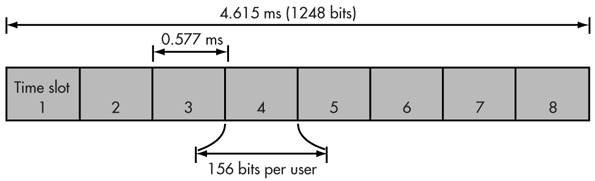
\includegraphics[width=0.82 \textwidth]{img/tdma.jpg}
\caption{TDMA: Elk tijdslot is toegewezen aan één gebruiker.}
\label{fig:tdma}
\end{figure}

\noindent 2G werd in 1991 commercieel gelanceerd in Finland. Deze 2G-telefoonsystemen verschilden van de vorige generatie in hun gebruik van digitale transmissie in plaats van analoge transmissie en ook door de introductie van geavanceerde en snelle telefoon-naar-netwerk signalering. De toename van het gebruik van mobiele telefoons als gevolg van 2G was explosief.\\ 

\noindent De tweede generatie introduceerde een nieuwe manier van communiceren. SMS-berichten werden mogelijk. Aanvankelijk enkel op GSM-netwerken maar uiteindelijk op alle digitale netwerken. Al snel werd SMS (Short Message Service) de communicatiemethode van de voorkeur bij de jeugd. Tegenwoordig geeft het grote meerderheid van mensen de voorkeur aan het verzenden van tekstberichten. Het aantal spraakoproepen daalt jaar na jaar.\\

\noindent Enkele voordelen van 2G zijn dat digitale signalen minder batterij vermogen verbruiken, dus het helpt mobiele apparaten om lang mee te gaan. Digitale codering verbetert ook de helderheid van het gesprek en vermindert ruis op de lijn. Digitale signalen worden als milieuvriendelijk beschouwd. Digitale codering heeft geheimhouding en veiligheid voor de gegevens- en spraak oproepen mogelijk gemaakt. Het gebruik van 2G-technologie vereist sterke digitale signalen om mobiele telefoons naar behoren te laten werken. \cite{2g}

\subsection{2.5G: GPRS}
General Packet Radio Service (GPRS) is een pakket georiënteerde standaard voor mobiele gegevens op GSM van het cellulaire communicatienetwerk. GPRS werd opgericht door het European Telecommunications Standards Institute (ETSI). In 2G-systemen levert GPRS-datasnelheden tot 114 kbit/s. \cite{2g} \\

\noindent GSM en GPRS maken gebruik van GMSK-modulatie. Gauss Minimum Shift Keying (GMSK), is een modulatie techniek die in verschillende digitale radiocommunicatiesystemen gebruikt wordt.\\

\noindent Voor GMSK zijn er twee hoofd technieken om de modulatie te genereren. De meest voor de hand liggende manier is om het modulatie signaal te filteren met behulp van een Gauss-filter, zie Figuur \ref{fig:gmsk01}. Vervolgens moet men dit toe passen op een frequentie modulator waarbij de modulatie-index is ingesteld op 0,5. Deze methode is heel eenvoudig en rechtlijnig. Het nadeel is dat de modulatie-index exact 0,5 moet zijn. Praktisch gezien is deze analoge methode niet geschikt omdat de component toleranties afwijken en niet exact kunnen worden ingesteld. Hierdoor zal er in de praktijk geen modulatie-index van exact 0,5 gehandhaafd kunnen worden. \cite{gmsk} \\

\begin{figure}[H]
\centering
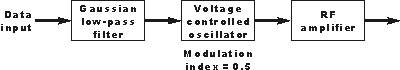
\includegraphics[width=0.85 \textwidth]{img/GMSK01.jpg}
\caption{GMSK met een Gauss-filter}
\label{fig:gmsk01}
\end{figure}

\noindent Voor GMSK-modulatie wordt wat bekend staat als een kwadratuur-modulator gebruikt. "The term quadrature means that the phase of a signal is in quadrature or 90 degrees to another one.'' Deze modulator gebruikt één signaal dat in fase is en een ander dat in kwadratuur staat. Dit type modulator wordt ook wel een I-Q-modulator genoemd, het blokdiagram hiervan is in Figuur \ref{fig:gmsk} te zien. Hiermee kan men de modulatie-index op exact 0,5 houden. Dit zonder dat er instellingen of aanpassingen nodig zijn. Voor de-modulatie kan de techniek in omgekeerde richting worden gebruikt. \cite{gmsk}

\begin{figure}[H]
\centering
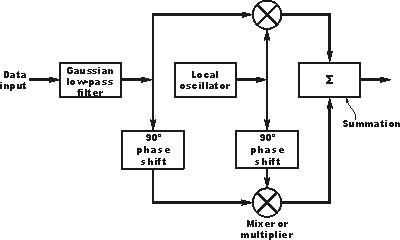
\includegraphics[width=0.85 \textwidth]{img/GMSK.jpg}
\caption{Blokdiagram van I-Q-modulator gebruikt om GMSK te maken}
\label{fig:gmsk}
\end{figure}



\subsection{2.75G: EDGE} \label{ssec:edge}
GPRS-netwerken zijn geëvolueerd naar EDGE-netwerken (Enhanced Data Rates for GSM Evolution) met de introductie van 8PSK-codering. EDGE werd vanaf 2003 ingezet op GSM-netwerken. Met EDGE werden snelheden tot 500 kbit/s mogelijk. \cite{2g} \\

\noindent 8-PSK (8 Phase Shift Keying), is een fase modulatie algoritme. Fase modulatie is een versie van frequentiemodulatie (FM) waarbij de fase van de draaggolf wordt gemoduleerd om bits van digitale informatie bij elke faseverandering te coderen.\\

\noindent De "PSK'' in 8-PSK verwijst naar het gebruik van Phased Shift Keying. Phased Shift Keying is een vorm van fase modulatie die wordt bereikt door het gebruik van een discreet aantal toestanden. 8-PSK verwijst dan logisch gezien naar PSK met 8 toestanden zoals men kan zien in het constellatie diagram op Figuur \ref{fig:8PSK}. Met de helft van dat aantal staten heb je QPSK (Quad Phase Shift Keying). Met tweemaal het aantal staten als bij 8-PSK, heb je 16PSK. Omdat QPSK 8 mogelijke toestanden heeft, kan 8-PSK drie bits per symbool coderen. 8-PSK is minder tolerant dan QPSK in het opzicht van slechte verbindingen, maar biedt meer data capaciteit. \cite{psk}


\begin{figure}[H]
\centering
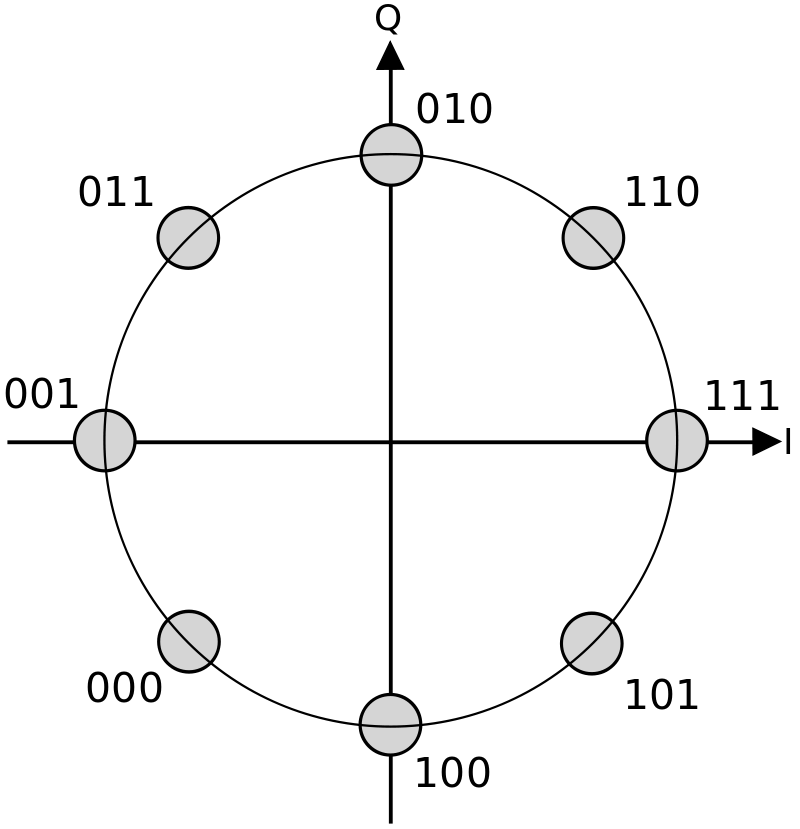
\includegraphics[width=0.75 \textwidth]{img/8PSK.png}
\caption{8PSK constellatie diagram}
\label{fig:8PSK}
\end{figure}


\section{3G: Hoge snelheid IP netwerk}
Toen het gebruik van 2G-telefoons wijdverspreid werd en mensen in hun dagdagelijks leven mobiele telefoons gingen gebruiken, werd het duidelijk dat de vraag naar datadiensten (zoals toegang tot internet) toenam. De 2G-technologie was niet meer voldoende dus begon de industrie te werken aan de implementatie van de volgende generatie technologie die beter bekend staat als 3G. Het belangrijkste technologische verschil dat 3G-technologie van 2G-technologie onderscheidt, is het gebruik van pakket schakeling in plaats van circuit schakeling voor gegevensoverdracht. \cite{3g} \\

\noindent Code-division multiple access (CDMA) is een digitaal kanaal toegang methode die wordt gebruikt door verschillende radiocommunicatie technologieën. CDMA is een voorbeeld van meervoudige toegang, waarbij verschillende zenders tegelijkertijd informatie kunnen verzenden over een enkel communicatiekanaal. Hierdoor kunnen verschillende gebruikers een band met frequenties delen.\\

\noindent Om dit mogelijk te maken zonder onnodige interferentie tussen de gebruikers gebruikt CDMA spread-spectrum technologie omdat het de gedigitaliseerde versie van een analoog signaal nodig heeft en het spreidt over een bredere bandbreedte op een lager vermogens-niveau. Het gedigitaliseerde en gecomprimeerde spraaksignaal in seriële gegevensvorm wordt verspreid door het in een XOF-schakeling te verwerken samen met een chipsignaal met een veel hogere frequentie. Dit kan men in Figuur \ref{fig:cdma} zien. De hoge verbindingssnelheid van 3G-technologie zorgden voor een transformatie in de industrie: voor het eerst werd mediastreaming van radio- en zelfs televisie inhoud voor 3G-handsets mogelijk. \cite{FDMA} \\

\begin{figure}[H]
\centering
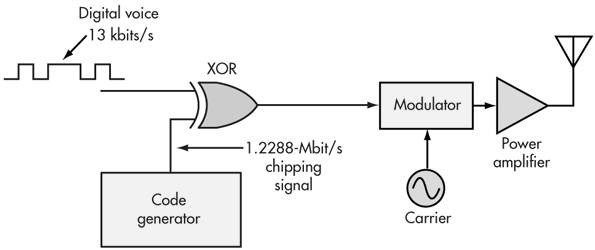
\includegraphics[width=0.75 \textwidth]{img/cdma.jpg}
\caption{CDMA signaal verwerking}
\label{fig:cdma}
\end{figure}

\noindent Zowel QAM als QPSK zijn modulatietechnieken die worden gebruikt in 3G draadloze technologieën. Voor QPSK kan men sectie \ref{ssec:edge} over PSK bekijken. De apparaten van de derde generatie, waaronder ook de LTE-apparaten vallen, gebruiken QPSK, 16QAM en 64QAM om gegevens te moduleren. Zie ook Figuur \ref{fig:qam}.\\

\noindent QAM (quadrature amplitude modulation) is een methode voor het combineren van twee amplitudegemoduleerde (AM) signalen in een enkel kanaal, waardoor de effectieve bandbreedte wordt verdubbeld. QAM wordt gebruikt met pulsamplitudemodulatie (PAM) in digitale draadloze toepassingen. In een QAM-signaal zijn er twee dragers, elk met dezelfde frequentie maar 90 graden in fase verschillend (een kwart van een cyclus, waaruit de term kwadratuur ontstaat). Eén signaal wordt het I-signaal genoemd en het andere wordt het Q-signaal genoemd. Wiskundig gezien kan een van de signalen worden gerepresenteerd door een sinusgolf en de andere door een cosinusgolf. De twee gemoduleerde draaggolven worden gecombineerd bij de bron voor transmissie. Op de bestemming worden de dragers gescheiden, de gegevens worden van elk geëxtraheerd en vervolgens worden de gegevens gecombineerd tot de oorspronkelijke gemoduleerde informatie. \cite{3gmod} \cite{qam}

\begin{figure}[H]
\centering
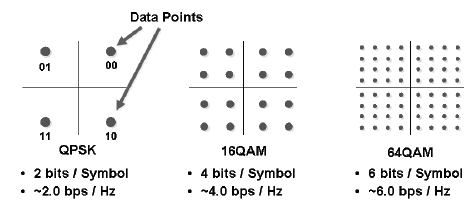
\includegraphics[width=0.85 \textwidth]{img/qam.png}
\caption{Modulatie technieken voor 3G}
\label{fig:qam}
\end{figure}

\subsection{3.5G: HSPA}
In het midden van de jaren 2000 begon een evolutie van 3G-technologie te worden geïmplementeerd, namelijk High-Speed Downlink Packet Access (HSDPA). Het is een verbeterd 3G-mobiel communicatieprotocol in de HSPA-familie (High Speed Packet Access), waarmee netwerken die zijn gebaseerd op Universal Mobile Telecommunications System (UMTS) hogere snelheden en capaciteiten hebben. \cite{3g}

\subsection{3.75G: HSPA+}
De verbeterde HSPA+ versie werd vrijgegeven in het najaar van 2008 met de daaropvolgende wereldwijde acceptatie in het begin van 2010. De nieuwere standaard maakt bit-rates mogelijk tot 337 Mbit/s voor de download en 34 Mbit/s voor de upload. Deze snelheden worden echter in de praktijk zelden bereikt. \cite{3g}

\subsection{3.9G: LTE} \label{ssec:lte}
In de telecommunicatie is Long-Term Evolution (LTE) een standaard voor high-speed draadloze communicatie voor mobiele apparaten en dataterminals. Deze is gebaseerd op de GSM/EDGE- en UMTS/HSPA-technologieën. Het verhoogt de capaciteit en snelheid met behulp van een andere radio-interface samen met netwerk verbeteringen.\\

\noindent LTE gebruikt dezelfde modulatietechnieken als de andere 3G generaties maar gebruikt een andere toegangsmethode. Orthogonal frequency-division multiple access (OFDMA) is een multi-user versie van het populaire orthogonale frequentie-deling multiplexing (OFDM) digitale modulatie schema. Multiple access wordt bereikt in OFDMA door subsets van subcarriers toe te wijzen aan individuele gebruikers (Figuur \ref{fig:ofdm}). Dit maakt gelijktijdige transmissie van lage datasnelheden van verschillende gebruikers mogelijk.
\cite{FDMA} \cite{3g}

\begin{figure}[H]
\centering
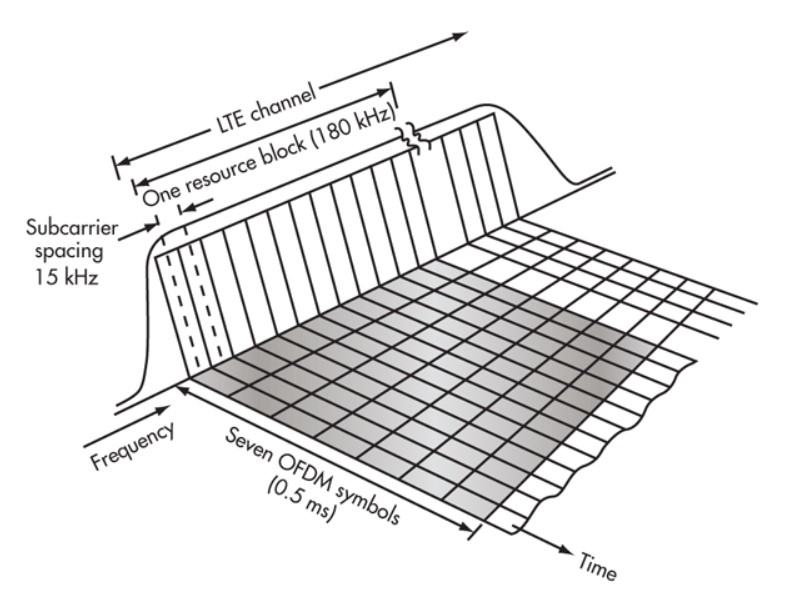
\includegraphics[width=0.85 \textwidth]{img/ofdm.jpg}
\caption{Visuele weergave van de subcarriers}
\label{fig:ofdm}
\end{figure}

\section{4G: Bandbreedte voor iedereen}

De industrie ging in 2000 al op zoek naar data geoptimaliseerde technologieën van de vierde generatie, met de belofte van snelheidsverbeteringen tot wel tien keer hoger dan bestaande 3G-technologieën. Het is eigenlijk de uitbreiding in de 3G-technologie met meer bandbreedte en dienstenaanbod in de 3G. De verwachtingen voor de 4G was in feite hoge kwaliteit audio en video streaming over een end-to-end internetprotocol. De vierde generatie kwam in 2010 voor het grote publiek beschikbaar.\\

\noindent De vierde generatie gaat verder op 3.9G en gebruikt net zoals LTE ook OFDM (zie sectie \ref{ssec:lte}).  4G gebruikt QPSK, 16QAM en 64QAM om gegevens te moduleren. Hierdoor denken velen dat LTE reeds 4G is ook al is het een deel van de derde generatie.\\

\noindent Een van de belangrijkste manieren waarop 4G technologisch van 3G verschilde, was de eliminatie van circuit switching. In plaats daarvan maakt 4G gebruik van een volledig IP-netwerk. 4G luidde een behandeling van spraakoproepen in met behulp van packet switching via internet, LAN of WAN netwerken via VoIP. Zo is een spraakoproep net als de rest een vorm van streaming. \\

\subsection{WIMAX}
WiMAX (Worldwide Interoperability for Microwave Access) was een kandidaat voor de 4G, in competitie met de LTE Advanced-standaard. Ze noemen WiMAX 4G, maar per definitie is WiMAX 3G. WiMAX biedt piekgegevenssnelheden van 128 Mbit/s als download en 56 Mbit/s als upload. \cite{3g} \cite{wimax}

\subsection{LTE-A} \label{ssec:LTE-A}
LTE-A definieert ook de werking van meerdere ingangen met meerdere uitgangen (MIMO) die meerdere zender-ontvanger antennes gebruikt. De datastream is verdeeld tussen de antennes om de snelheid te verhogen en om de link betrouwbaarder te maken. Met behulp van OFDM en MIMO laat LTE-A gegevens leveren met een snelheid van 100 Mb/s als download en 50 Mb/s als upload onder de beste omstandigheden. \cite{3g}

\section{5G: Lage latency}
Het 5G-netwerk is de volgende generatie mobiele netwerken en bieden hogere snelheden en betrouwbaardere verbindingen op smartphones en andere apparaten. De combinatie van geavanceerde netwerktechnologieën en het allernieuwste onderzoek zorgt ervoor dat 5G verbindingen naar verwachting een gemiddelde download snelheden van ongeveer 1GB/s zouden kunnen halen. De netwerken zullen een explosieve toename van de IOT (Internet Of Things) technologie mogelijk maken en de infrastructuur bieden die nodig is om enorme hoeveelheden data te vervoeren, waardoor een slimmere en meer verbonden wereld mogelijk wordt. Naarmate de ontwikkeling vordert, zullen naar verwachting 5G-netwerken over de hele wereld worden gelanceerd in 2020. \cite{5g}


\subsection{Focus punten}
De hoofd toepassingen voor 5G (Figuur \ref{fig:5g}) zijn onder te verdelen in drie categorieën: Enhanced mobile broadband (eMBB) voor verbluffende multimedia-ervaringen, Ultra-Reliable Low-Latency Communication (URLLC) voor bedrijfskritieke apparaat besturing en Massive machine type communication (mMTC) voor IOT (Internet Of Things) toepassingen.

\begin{figure}[H]
\centering
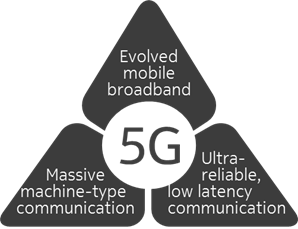
\includegraphics[width=0.80 \textwidth]{img/5g.png}
\caption{De drie focus punten van 5G.}
\label{fig:5g}
\end{figure}

\subsubsection{Enhanced mobile broadband (eMBB)}
eMBB is één van de drie pilaren waarop 5g rust. Het verwijst naar het gebruik van 5G als een evolutie van 4G LTE. Met een snellere verbinding, hogere doorvoer en meer capaciteit moet eMBB (5G) zich onderscheiden van 4G LTE. Het streamen van media op hoge resoluties en hoge bitrates, web-browsing gelijk op een vaste verbinding en zelfs cloud gaming behoren tot de mogelijkheden. \cite{spec} \cite{urllc} \cite{5gc}

\subsubsection{Ultra-Reliable Low-Latency Communication (URLLC)}
De volgende pilaar is URLLC. Vele toepassingen hebben strikte eisen voor latency en betrouwbaarheid. Voor operaties op afstand, autonome voertuigen en fabriek automatisaties, allemaal situaties waarbij communicatie betrouwbaar en snel moet zijn mag er niets mis lopen. Hierdoor komt URLLC met wachttijden van minder dan een milliseconde en met een fouten marge van lager dan één pakket per 100000 ($10^5$) pakketten. \cite{spec} \cite{urllc} \cite{5gc}

\subsubsection{Massive machine type communication (mMTC)}
Tot slot is er nog de mMTC pilaar. Met mMTC moet 5G smallband internettoegang voor een zeer groot aantal apparaten op een zeer klein oppervlak gaan ondersteunen. Deze apparaten kunnen detectie-, meet- of bewakingsapparatuur zijn. Het omvat dus apparaten die kleine hoeveelheden data sporadisch of in bepaalde intervallen versturen. Dit zijn de zogenaamde IOT toepassingen. \cite{spec} \cite{urllc} \cite{5gc}


\subsection{Technologieën}
Meer snelheid met lagere latency dat is wat er van 5G verwacht wordt. De technologieën die het mogelijk maken worden hieronder beschreven. In het kort beschreven zal 5G gebruik maken van verschillende frequentie domeinen om snelheid op hotspots te kunnen halen maar ook om op langere afstand nog steeds bereik te hebben. De OFDM techniek blijft behouden maar wordt aangevuld met DFT-s-OFDM (discrete Fourier transform spread orthogonal frequency division multiplexing) alsook 256-QAM. DFT-s-OFDM verminderd de kans op interferentie bij lage zendvermogens en gaat enkel voor upload ingezet worden.

\subsubsection{Radio Frequenties en Modulatie}
De vijfde generatie gaat gebruik maken van twee frequentie domeinen. Enerzijds het sub 6 GHz (FR1) domein en anderzijds het domein van 24 GHz tot 86 GHz (FR2). \cite{5gband} \\

\noindent De maximale bandbreedte per kanaal voor het sub 6 GHz frequentie domein is 100 MHz. Merk op dat LTE 100 MHz draaggolf-aggregatie (vijf x 20 MHz-kanalen) ondersteunt. FR1 ondersteunt een maximaal modulatie formaat van 256-QAM terwijl LTE een maximum van 64-QAM heeft, wat betekent dat 5G aanzienlijke doorvoer verbeteringen realiseert ten opzichte van LTE in de sub-6 GHz-banden. \cite{5gband} \cite{5gmodulation} \\

\noindent De maximale bandbreedte per kanaal is voor FR2 gedefinieerd op 400 MHz. De maximale snelheid die mogelijk door deze configuratie wordt ondersteund, is ongeveer 40 Gbit/s. In Europa is 24,25 GHZ tot 27,5 GHz het voorgestelde frequentiebereik voor FR2. \cite{5gband}\\

\noindent Voor OFDM met cyclische prefix (CP) gebruikt men voor zowel downloaden als uploaden: QPSK, 16QAM, 64QAM en 256QAM als modulatiemethoden. De DFT-s-OFDM met cyclische prefix (CP) gebruikt men enkel voor upload. Hierbij gebruikt men $\pi$/ 2-BPSK, QPSK, 16QAM, 64QAM en 256QAM als modulatiemethoden. 3PP-discussies zijn bezig met betrekking tot de ondersteuning van 1024QAM. \cite{5gmodulation}\\



\subsubsection{MIMO}
Zoals eerder aangehaald in sectie \ref{ssec:LTE-A} is MIMO het gebruik van meerdere antennes. Meerdere input en meerdere outputs vergroten de doorvoer en de capaciteits dichtheid met behulp van grote aantallen antennes. De term "massieve MIMO" werd voor het eerst bedacht door Nokia Bell Labs-onderzoeker Dr. Thomas L. Marzetta in 2010 en werd gelanceerd in 4G-netwerken. \cite{mimo}




\section{Conclusie}
Door de jaren heen is de technologie voor mobiele communicatie enkel maar verbeterd. Enorme verbeteringen op vlak van snelheid, latency, energie verbruik en prijs komen gepaard met iedere nieuwe generatie. Voordat een nieuwe generatie commercieel uitrolt is men reeds bezig met de volgende generatie. Dit kan men zien op Figuur \ref{fig:evolution}. Hier is duidelijk op te zien hoe de uitrol van een nieuwe generatie gelijk loopt met de ontwikkeling van de volgende.\\

\noindent Naar de toekomst toe zal er steeds meer ingezet worden op lage latency, hoge snelheid met lage foutmarges en lage packet-loss. 5G is nog niet commercieel uitgerold en dat maakt het perfect om nu al na te denken over de volgende generatie. Generatie 6 is reeds in ontwikkeling en wilt geen milliseconden latency maar microseconden latency gaan aanbieden.\\




\begin{figure}[H]
\centering
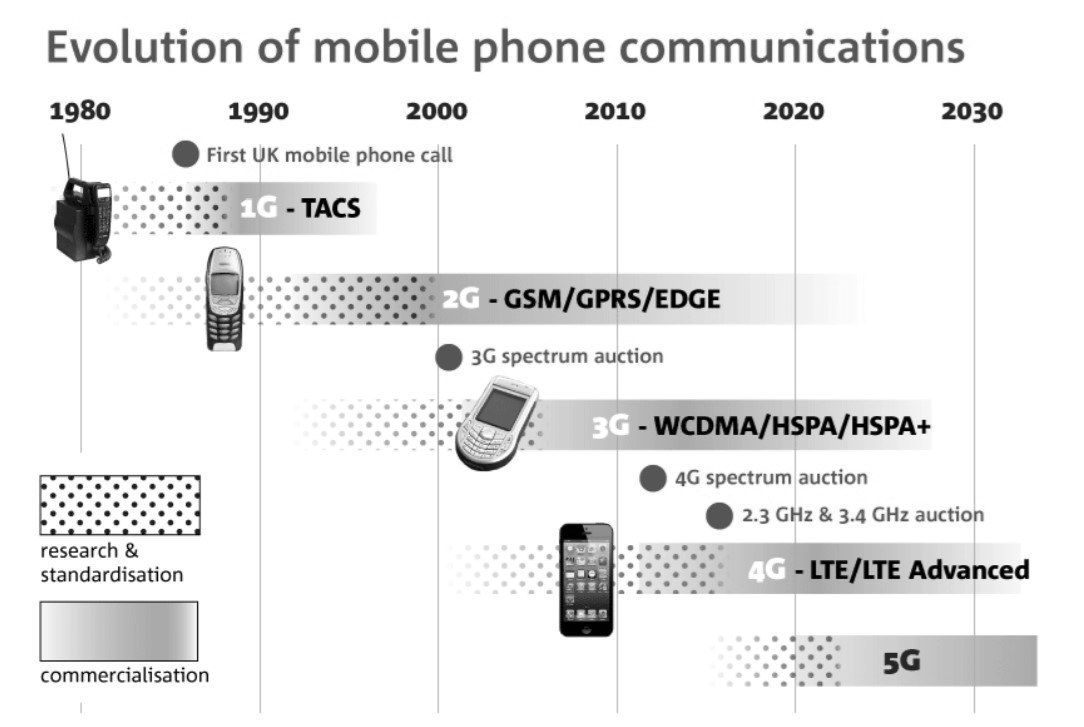
\includegraphics[width=0.95 \textwidth]{img/evolution.jpg}
\caption{De evolutie van de verschillende generaties doorheen de jaren.}
\label{fig:evolution}
\end{figure}
\newpage

\bibliographystyle{ieeeconf}
\begin{thebibliography}{9}

\bibitem{0G} 
Clear Doubts - What is Mobile Radio Telephone System or 0G?\\
\texttt{http://www.cleardoubts.com/technology/\\what-is-mobile-radio-telephone-system-or-0g-and-what-is-0-5g/} \\Jul. 27, 2011 [Dec. 11, 2018]. 

\bibitem{FDMA} 
Access Technologies: FDMA, TDMA, CDMA, OFDMA, AND SDMA  \\
\texttt{https://www.electronicdesign.com/communications/fundamentals-\\communications-access-technologies-fdma-tdma-cdma-ofdma-and-sdma} \\Jan. 22, 2013 [Dec. 11, 2018]. 

\bibitem{fm} 
Frequency Modulation\\
\texttt{https://fas.org/man/dod-101/navy/docs/es310/FM.htm} \\ Onbekend [Dec. 11, 2018]. 


\bibitem{1G} 
archive.today - 1G: First Generation wireless technology  \\
\texttt{https://archive.is/20130103094947/http://www.javvin.com/\\wireless/1G.html}\\ Jan. 03, 2013 [Dec. 12, 2018]. 


\bibitem{technieken}
Technologies used in 1G or First generation of Wireless Telecommunication\\
\texttt{http://www.cleardoubts.com/technology/technologies-used-in-1g-or-\\first-generation-of-wireless-telecommunication-technology/} \\Dec. 03, 2011 [Dec. 13, 2018]. 

\bibitem{amps} 
Advanced Mobile Phone System (AMPS)\ -  Cellular Telephone Systems\\
\texttt{http://www.wirelesscommunication.nl/reference/chaptr01/telephon/amps.htm} \\1995 [Dec. 17, 2018]. 

\bibitem{nokia} 
Himanshu - The rise, dominance, and epic fall\\
\texttt{https://www.gsmarena.com/the\_rise\_dominance\_and\_epic\_fall\_a\_brief\_\\look\_at\_nokias\_history-blog-13460.php} \\Aug. 12, 2015 [Dec. 17, 2018]. 

\bibitem{2g} 
Ai Sin Chan  - A brief history of 2G mobile communication technology\\
\texttt{https://blog.xoxzo.com/en/2018/08/01/history-of-2g/} \\Jan. 08, 2018 [Dec. 18, 2018]. 

\bibitem{gmsk} 
Ian Poole - What is GMSK Modulation - Gaussian Minimum Shift Keying\\
\texttt{https://www.radio-electronics.com/info/rf-technology-design/pm-phase-modulation\\/what-is-gmsk-gaussian-minimum-shift-keying-tutorial.php} \\Onbekend [Dec. 18, 2018].

\bibitem{psk} 
Ian Poole - What is PSK, Phase Shift Keying\\
\texttt{https://www.radio-electronics.com/info/rf-technology-design/pm-phase-modulation\\/what-is-psk-phase-shift-keying-tutorial.php} \\Onbekend [Dec. 18, 2018].

\bibitem{3g} 
Lou Frenzel - What’s the Difference Between 3G and 4G Cellular Systems?\\
\texttt{https://www.electronicdesign.com/4g/what-s-difference-between-3g-and-4g\\-cellular-systems}\\ Jan. 25, 2012 [Dec. 21, 2018].

\bibitem{3gmod} 
Mohamed Abdel Monem - Modulation and Signal Quality at LTE\\
\texttt{https://www.netmanias.com/en/post/blog/12441/lte/modulation-and-signal-\\quality-at-lte}\\ Jul, 28 2017 [Dec. 21, 2018].

\bibitem{qam} 
Ian Poole - What is QAM - Quadrature Amplitude Modulation\\
\texttt{https://www.radio-electronics.com/info/rf-technology-design/quadrature-\\amplitude-modulation-qam/what-is-qam-tutorial.php}\\ Onbekend [Dec. 21, 2018].

\bibitem{wimax} 
Wegwijs in frequentieland - WiMaX\\
\texttt{http://www.frequentieland.nl/draadloos/wimax.htm}\\Onbekend [Dec. 21, 2018].

\bibitem{5g} 
SDX Central - Key Elements for the 5G Network\\
\texttt{https://www.sdxcentral.com/5g/definitions/key-elements-5g-network/} \\Onbekend [Dec. 25, 2018].

\bibitem{spec} 
MediaTek - 5G: What are eMBB, URLLC and mMTC?\\
\texttt{https://www.mediatek.com/blog/5g-what-are-embb-urllc-and-mmtc} \\
Mar, 08 2018 [Dec. 25, 2018].

\bibitem{urllc} 
EventHelix - Ultra-Reliable Low-Latency Communication\\
\texttt{https://medium.com/5g-nr/ultra-reliable-low-latency-communication-\\urllc-9b2505e81579}\\ May, 28 2018 [Dec. 25, 2018].

\bibitem{5gc} 
Ellen Warren - 5G is totally changing how we connect\\
\texttt{https://www.nokia.com/blog/5g-totally-changing-how-we-connect/} \\
Mar, 16 2018 [Dec. 25, 2018].

\bibitem{5gband} 
5G Frequency Bands \& Spectrum Allocations\\
\texttt{https://www.cablefree.net/wirelesstechnology/4glte/5g-frequency-bands-lte/} \\Onbekend [Dec. 25, 2018].

\bibitem{5gmodulation} 
MediaTek - 5G: Break down the essentials of Waveform and Multiple Access\\
\texttt{https://www.mediatek.com/blog/5g-breaking-down-the-essentials-of-its-\\waveform-and-multiple-access} \\
Mar. 9, 2018 [Dec. 29, 2018].

\bibitem{mimo} 
Massive MIMO– Gives large capacity gain, coverage, and energy efficiency\\
\texttt{https://networks.nokia.com/solutions/massive-mimo} \\
Onbekend [Dec. 29, 2018].



\end{thebibliography}

\end{document}
